\chapter{Generic Heuristics Framework}
\label{chapter3}

In this chapter, is intended to perform a detailed description of the generic framework here created, in order to test the different heuristic algorithms developed along this dissertation. This chapter begins by providing a global description of the created framework in section \ref{general_description} and by presenting a flowchart explaining how it works. In the remaining sections, a detailed description is provided on every individual main entity of the framework. In section \ref{scheduler} is addressed the scheduler block, in section \ref{logicalTopologyGenerator} the logical topology generator, in section \ref{physicalTopologyGenerator} the physical topology generator, in subsection \ref{logicalTopologyManager2} the logical topology manager and finally, in section \ref{physicalTopologyManager} the physical topology manager. 

\section{General Description}
\label{general_description}
The key role of frameworks, in general, is to permit developers to address only project relative needs rather than the low level phases of working systems, resulting in reduced times for development tasks. Speaking more specifically about the framework here created, it consists in a conceptual structure composed of a set of different layered entities which provide generic functionality while also being able to be selectively changed, thus enabling the possibility of future improvement by introducing new and more complex features and considerations of real worldwide networks. This framework was intended to serve as a support for the complex  problem of dimensioning optical transparent networks. In figure \ref{framework} a top level diagram of the developed platform, in which the heuristic algorithms were later implemented, is provided. In this flowchart, as well as for the remaining in this chapter, the rectangle shapes represent the main entities of the framework, the diamond shapes symbolize decision points and the rounded rectangle shapes symbolize the system entry parameters.
\clearpage

\begin{figure}[H]
  \begin{center}
    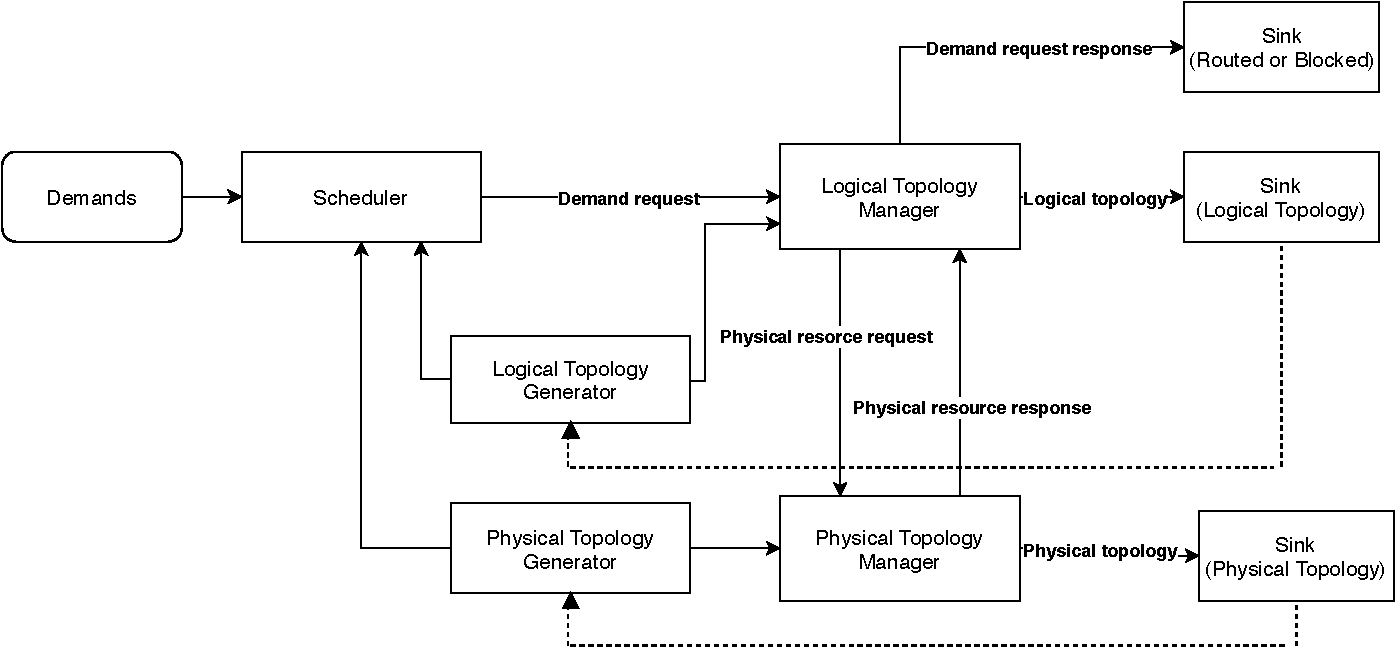
\includegraphics[width=1\textwidth]{fig/logos/framework.pdf}
    \caption{Top level diagram of the developed framework. The solid lines represent vital connections between blocks as well as the flow of information, on the other hand, the dashed lines represent possible but non obligatory connections, since the framework runs correctly with or without them. They provide the possibility of starting a simulation by creating a void physical and/or logical topology or to load a previous state.}
  \end{center}
  \label{framework}
\end{figure}

When there is one or multiple traffic demands to be processed initially they must be sorted in a scheduler block, according to a predefined rule. Thereafter, the demands are sent one by one into a logical topology manager block where either an already existent capacity is used to route the demand or a request is made to create the capacity. That request is sent to a physical topology manager, where the information about the network physical links capacity is stored, and depending on the existence of remaining capacity, between other aspects, a response is given back to the logical topology manager regarding the possibility or not to route the demand. Finally, the useful information contained on the logical and physical manager blocks, as well as the information regarding the status of each processed demand, can be stored in sink blocks also presented in the diagram above.    

\section{Scheduler}
\label{scheduler}

  When using global optimization techniques such as integer linear programming, the order of the demands becomes not relevant, once every possible scenario is tested, however, this is not the case since in this dissertation we are considering heuristic approaches. Having that said, before the traffic demands can be processed a scheduler block is needed, which will be responsible for the creation of an ordered queue based on specific predefined criteria. That same order becomes the order by which demands will be processed, and so ultimately routed or blocked. Demands can be sorted in many different ways when recurring to different strategies, which may potentially affect the efficiency of the routing and grooming processes. Therefore, different methods usually also have different impacts on the cost of the network, the loading in the network and the blocking probability.
  
  %Those strategies may rely individually on the quantity of traffic of each individual request, the traffic granularity, the length of the shortest logical or physical paths either in terms of distance or hops, the need of protection paths, the quality of the path set in terms of desirable path options or a smart combination of some of this aspects \cite{SimmonsJane2008}. Other ordering strategies are also possible but in general none of them reclaims the best results for every practical scenario.
  
  
  
\section{Logical Topology Generator}
\label{logicalTopologyGenerator}

Based on the physical topology adjacency matrix of the network and the transport mode utilized a new upper layer can be created, the logical topology. Each node may be optical directly connected to each other, only optical connected to adjacent nodes or optical connected to suitable nodes. Between directly interconnected nodes a lightpath can be established, in which the information is carried. This variety of possible optical paths along the route imposed by logical topology lead to a situation of three possible transport modes: opaque, transparent or translucent \cite{Vasco}. In this block the initial logical topology must be created and sent to a logical topology manager block where the routing and grooming heuristic algorithms, that depend directly of the logical topology, are implemented and will be continually updated as demands are processed. Once again, the dashed lines presented in figure \ref{framework} symbolize the ability of a logical topology generator block to create the logical topology either void, when no previous information is provided, or by loading a previous network state, where there were already demand requests being supported and as such some lightpaths had already been established.  

\section{Physical Topology Generator}
\label{physicalTopologyGenerator}

Here, is created the initial physical layer of the network. It consists mainly in a set of physical links, which may interconnect a pair of nodes and can be expressed as being uni or bidirectional, in such a way, that each of the transmission systems that support the links are comprised of a unique fiber or a pair of fibers transmitting in opposite directions, respectively. Once more, the dashed lines presented in figure \ref{framework} symbolize the ability of a physical topology generator block to also create the physical topology either void, when no previous information is provided to it, or by loading a previous network state where there were already demand requests being supported and as such some physical capacity had already been reserved.

\section{Logical Topology Manager}
\label{logicalTopologyManager2}

In this block the initial logical layer, originating from a logical topology generator block, is stored and continuously updated as demands are processed. The grooming and part of the routing algorithms should be implemented here and they can assume many different strategies. The current logical layer state of the network is accessible from this block and can contain information of the existent paths and the respective lightpaths that comprise them, between others. While processing a demand if there is no available path available for it then a new should be selected, based on a defined routing strategy, and a request sent to the physical topology manager in order to verify the possibility of establishing that path. Depending on the physical topology manager response either a path is created and the demand routed or, in the case it is not possible to do so, the demand remains blocked.  Only a demand request serves as input for this entity but on the other hand the outputs can differ as they can represent a request to establish a new path, sent to the physical topology manager of the network, or simply the information about whether or not a demand was routed, sent to a sink block. 

\begin{figure}[H]
  \begin{center}
    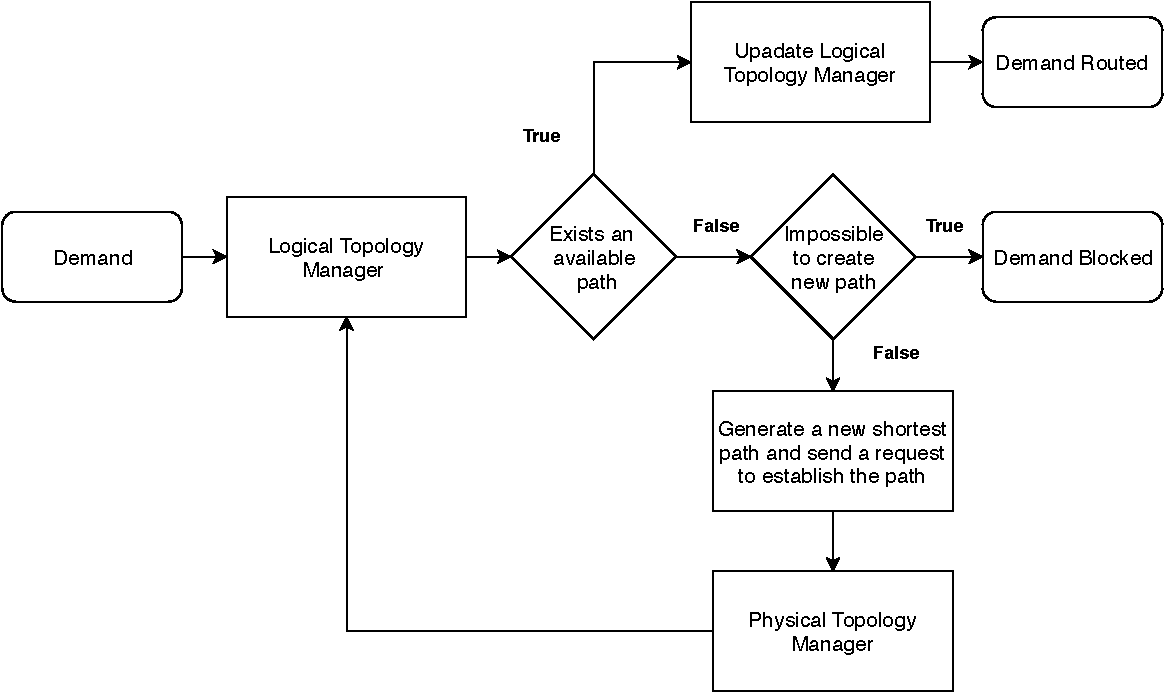
\includegraphics[width=1\textwidth]{fig/logos/LogicalTopologyManager.pdf}
    \caption{Flowchart representing the interaction between the logical and physical topology manager entities while processing a demand request.}
  \end{center}
  \label{logicalTopologyManager}
\end{figure}

\section{Physical Topology Manager}
\label{physicalTopologyManager}

The main function of this block is to administrate the physical layer of the network and inform the logical topology manager of the available physical capacities of all the links necessary to establish paths. When a path is selected for a demand in the logical layer, through a routing algorithm, a request is made for it and sent here. That path must be broken into sub-connections, i.e. lightpaths, if necessary, and each of the lightpaths assigned with a wavelength if possible. Thus, the wavelength assignment strategy should be applied here. The need of wavelength continuity arises for optical-bypass-enabled networks and as such, this property is tightly coupled to the routing process, as the selection of the route determines the links on which a free wavelength must be found \cite{SimmonsJane2008}. However, there is the possibility of none feasible wavelength to be found for one or more of the lightpaths, resulting in the occurrence of the wavelength contention phenomenon. Due to the possible loss of network efficiency, caused by wavelength contention situations, this is a problem that must be carefully addressed. 

%\section{Sink}
%\label{sink}

%Here the final states of the network can be stored. Three blocks are in need, a first to record the demands processed and two others for the logical and physical layer states of the network. The information about every traffic demand processed can be stored here, where each demand must be properly identified as well as its status (routed or blocked). Additionally, in the case it has been successfully routed the path taken must also be identified. The final values of the logical and physical topologies of the network are also to be stored so that they can be consulted at any time. Combining all this information it is possible to trace the routing scheme of all the processed traffic. 

\section{Chapter summary}

In this chapter are introduced some concepts regarding the created framework and the constituting entities are summarize in terms of features and possibilities provided. A flowchart is also provided where is represented the interaction between the two main entities of the framework (logical and physical topology managers), while processing a single traffic request. Although in this dissertation, is only addressed the problem of transparent networks, it is important to notice that the framework was developed to allow a more generic use, it provides the possibility of future improvements in order to contemplate other realistic network scenarios, for example other transport modes or the existence of protected traffic.

\cleardoublepage